\documentclass{article}
\usepackage{graphicx}
\graphicspath{ {./static} }
\author{Evan Dreher}
\title{Overview}

\begin{document}
\section{Gameplay}
\par The game hnefatafl is shrouded in some level of mystery since no official rules were ever documented for it. Here are the rules this implementation will be using.

\subsection{Setup}
\begin{enumerate}
	\item The game will be played on an $11\times 11$ board. The center square and the corner squares will be "king squares" (see TODO)
	\item The white king will be start the game on the center square.
	\item The 12 white knights will start on the 12 squares that are a unit distance of 2 away from the center square where the king is.
	\item The 5 center squares of each edge of the board will have 5 black knights on them and an additional black knight will be placed on the centermost square by each edge of the board at a depth of one such that after all the pieces are set up, the board will look like this.	
\end{enumerate}
\begin{center}
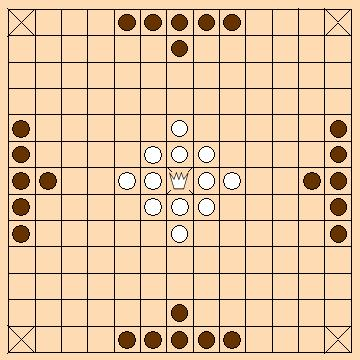
\includegraphics[height=40ex]{Board}
\end{center}
\subsection{
\end{document}
